\documentclass[t]{beamer}
\usepackage{beamerthemeiut}
\usepackage[T1]{fontenc}
\usepackage{graphicx}
\usepackage{epstopdf}
\usepackage{amsfonts,amssymb,amsmath} %package math
\usepackage{txfonts}
\usepackage{subcaption}
\captionsetup{compatibility=false}

\definecolor{color1}{RGB}{255, 178, 178}
\definecolor{color2}{RGB}{178, 178, 255}
\definecolor{color3}{RGB}{236, 217, 198}


\setbeamertemplate{theorems}[numbered]
\setlength{\abovecaptionskip}{1ex}

\title{Le titre de ma pr�sentation}
\author{Mon nom Mon prenom}
\institute{IUT de Brest}
\date{}
\setbeamercolor{alerted text}{fg=red} 
\setbeamercovered{transparent}
\setcounter{tocdepth}{2}     %% Visibles dans la table des matieres

\begin{document}
\setbeamertemplate{background canvas}{
\includegraphics[width=\paperwidth,height=\paperheight]{fond_iut_1.pdf}}

%premier slide
    \begin{frame}[plain]
    \vskip 2cm
    \titlepage
    \end{frame}

\setbeamertemplate{background canvas}{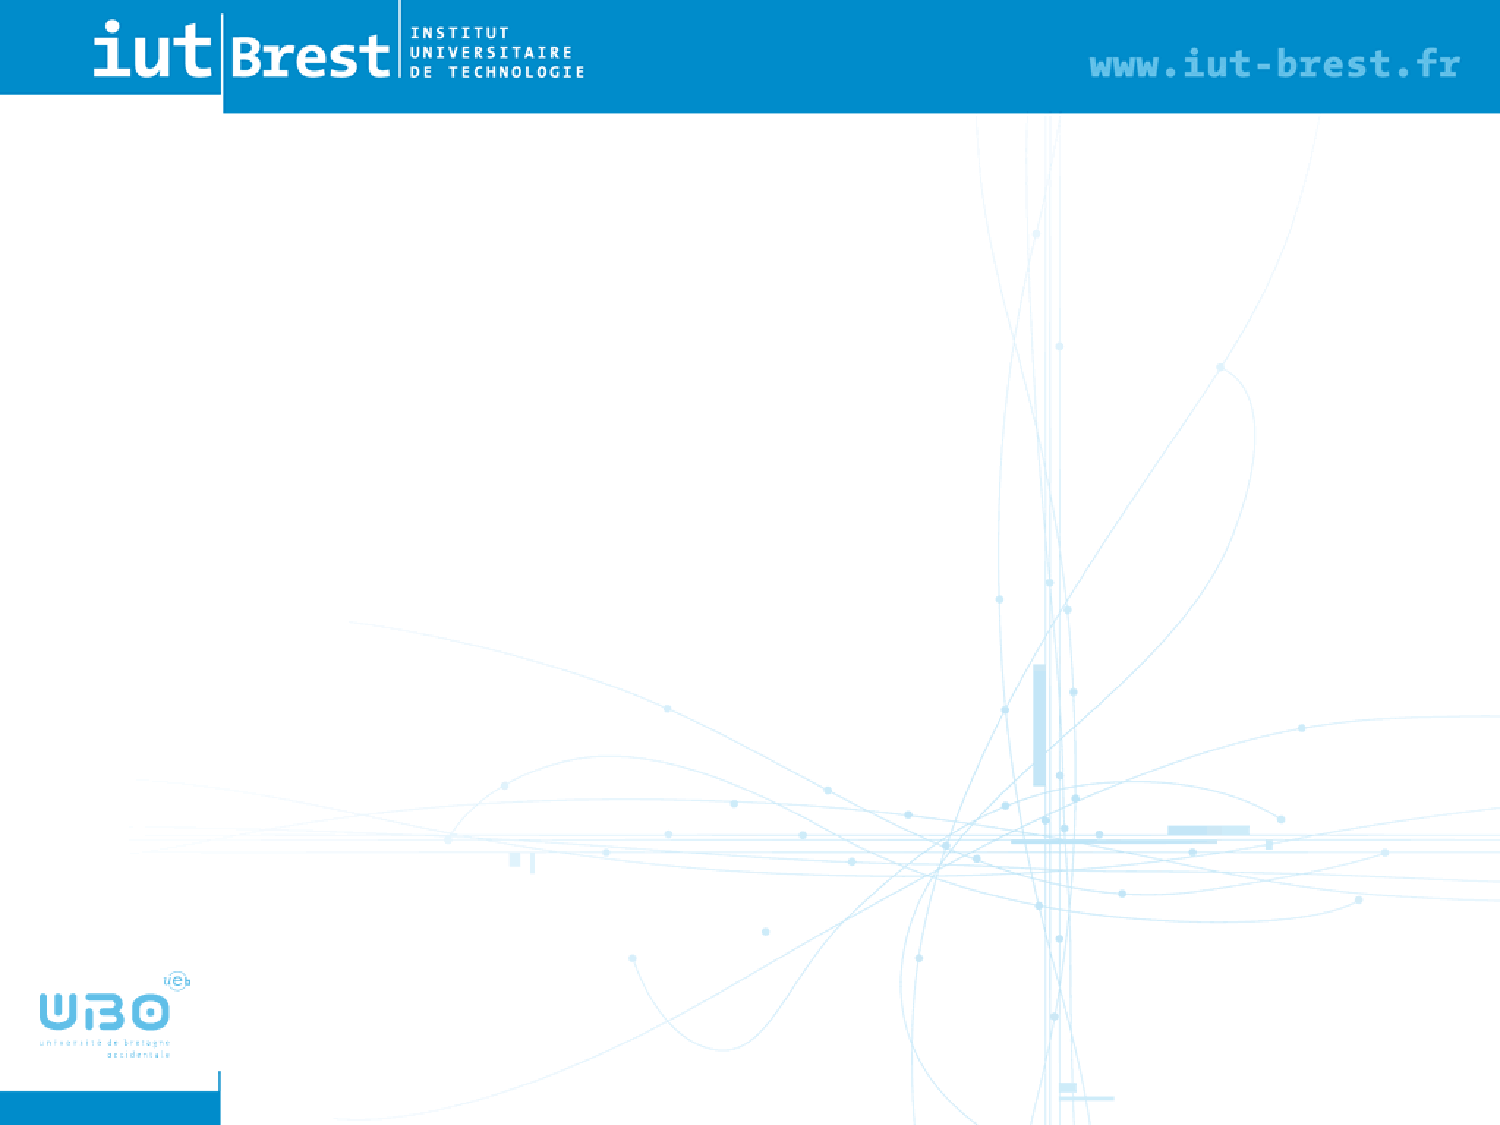
\includegraphics[width=\paperwidth,height=\paperheight]{fond_iut_2.pdf}}

%table des mati�res
\section*{Plan de la pr�sentation}

\begin{frame}
   	\frametitle{\insertsection}
	\hskip 0.4cm
    	\begin{minipage}[c]{.95\linewidth}
    		\color{bleu2}
   		\tableofcontents
     	\end{minipage}
 \end{frame}

%Autres slide
\section{Rappels}
\subsection{Dat�s Cl�s}

\begin{frame}{\insertsection - \insertsubsection}
	\begin{itemize}
	\item 2006: La licence professionnelle "�lectronique \& Informatique des syst�me Industriels" (EISI) est cr��e. Cette licence comporte deux options: "Syst�mes Automatis�s et
	R�seaux Industriels" et "�lectrotechnique et �lectronique de Puissance".
	\item 2008: Suite � la campagne de r�habilitation de 2007, la licence professionnelle EISI est d�coup�e en deux licences professionnelles nomm�es respectivement SARI et EEP. 
	\item 2011: La licence SI-SARI obtient la note A lors de la campagne d'�valuation de l'AERES 2010-2011.
	\item 2015: La sp�cialit� SI-SARI sera remplac�e par la mention "\alert{Syst�mes Automatis�s, R�seaux, Informatique Industrielle}" (SARII) lors de la rentr�e 2015.
	\end{itemize}
\end{frame}

\subsection{Contexte National}

\begin{frame}{\insertsection - \insertsubsection}
	\begin{figure}[!h]
	\centering
	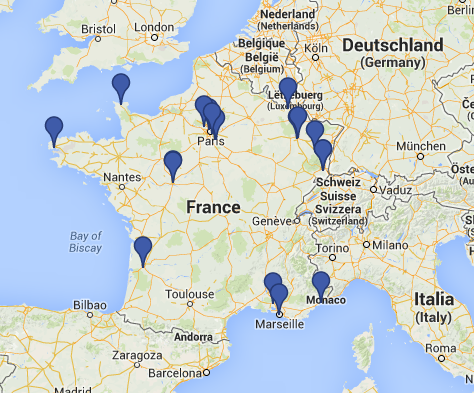
\includegraphics[width=7cm]{./figure/SARI.png}
	\caption{Emplacement g�ographique des licences SARI}.
	\end{figure}
\end{frame}

\subsection{Transform�e de Fourier}

\begin{frame}{\insertsection - \insertsubsection}
	\begin{itemize}
	\item La transform�e de Fourier:
	\begin{align}
	X(f)&=\int_{-\infty}^{\infty}x(t)e^{-2j\pi ft}dt
	\end{align}
	\visible<2->{  %D�masquage au deuxi�me sous-slide
	\item La transform�e de Fourier \alert<3>{Inverse}:
	\begin{align}
	x(t)&=\int_{-\infty}^{\infty}X(f)e^{2j\pi ft}df
	\end{align}}
	\end{itemize}
\end{frame}


\end{document}
